Il seguente processo contiene le attività che sovraintendono alla costruzione del prodotto software da parte del team \GRUPPO. 

\subsubsection{Analisi dei requisiti}
E' compito degli \textit{Analisti} stilare il documento \textit{Analisi dei requisiti}.
In questo documento dovranno essere presenti tutti i requisiti ed i \gls{casi d'uso} emersi dall'analisi del capitolato e dalle riunioni con il Proponente.\\

\subsubsection{Requisiti}

I requisiti dovranno essere classificati per tipo e priorità, utilizzando la seguente notazione:

\begin{center}
\begin{math}
R \left [ importanza \right ] \left [ tipo\right ]\left [codice\right ]
\end{math}
\end{center}
\begin{itemize}
  \item Importanza può assumere i seguenti valori:
\begin{itemize}
	\item \textbf{OBB:} Requisito obbligatorio;
	\item \textbf{DES:} Requisito desiderabile;
	\item \textbf{OPZ:} Requisito opzionale.
\end{itemize}
  \item Tipo può assumere i seguenti valori:
\begin{itemize}
	\item \textbf{F:} Requisito funzionale;
	\item \textbf{Q:} Requisito di qualità;
	\item \textbf{P:} Requisito di prestazione;
	\item \textbf{V:} Requisito di vincolo.
\end{itemize}
  \item Codice rappresenta il codice univoco di ogni requisito in forma gerarchica.
\end{itemize}
Ogni requisito dovrà essere inserito (nel documento \textit{Analisi dei Requisiti}) in una tabella contenente il codice identificativo, una breve descrizione e la fonte.

\subsubsection{Casi d'uso}

Dopo la stesura dei requisiti è sempre compito degli analisti analizzare i \gls{casi d'uso} (abbreviati con UC, use case).
Per ogni caso d'uso sono richieste le seguenti informazioni:
\begin{itemize}
	\item \textbf{Attori:} gli attori coinvolti nel caso d'uso (principali e secondari);
	\item \textbf{Scodo e descrizione:} una breve descrizione chiara e dettagliata del caso d'uso;
	%\item Codice identificativo: nel formato UCxx, dove xx indica un numero identificativo del caso d'uso;
	%\item Titolo: titolo sintetico del caso d'uso;
	\item \textbf{Precondizione:} la precondizione del requisito;
	\item \textbf{Flusso degli eventi:} specificare per ogni evento: descrizione, attori coinvolti e se lo scenario è descritto in dettaglio da un altro caso d'uso;
	%\item Diagramma: dovrà essere usato \gls{UML} 2.4 per la creazione dei diagrammi dei \gls{casi d'uso};
	\item \textbf{Postcondizione:} la postcondizione del requisito.
\end{itemize}
\newpage
\subsubsection{Tracciamento}
Per il tracciamento dei requisiti è stato creato un \gls{database} che tiene traccia dei requisiti, \gls{casi d'uso} e tutte le dipendenze.
È stato realizzato un \gls{plugin} per il Content Management System (\gls{CMS}) \gls{WordPress} per rendere possibile il popolamento e l'interrogazione.
Il \gls{plugin} genera automaticamente il codice \LaTeX\ per l'\textit{Analisi dei Requisiti}.
Per sua natura, il \gls{plugin} è portabile su tutte le versioni di \gls{WordPress} ed alla fine del progetto sarà reso open-source in modo che possa essere riutilizzato da chi lo desideri. È stato scelto questo \gls{CMS} poiché, essendo conosciuto da due membri del gruppo, permette di concentrarsi esclusivamente sulla gestione dei requisiti tralasciando tutti gli aspetti di contorno, comprimendo così notevolmente i tempi di sviluppo.
\begin{figure}[h]
\centering
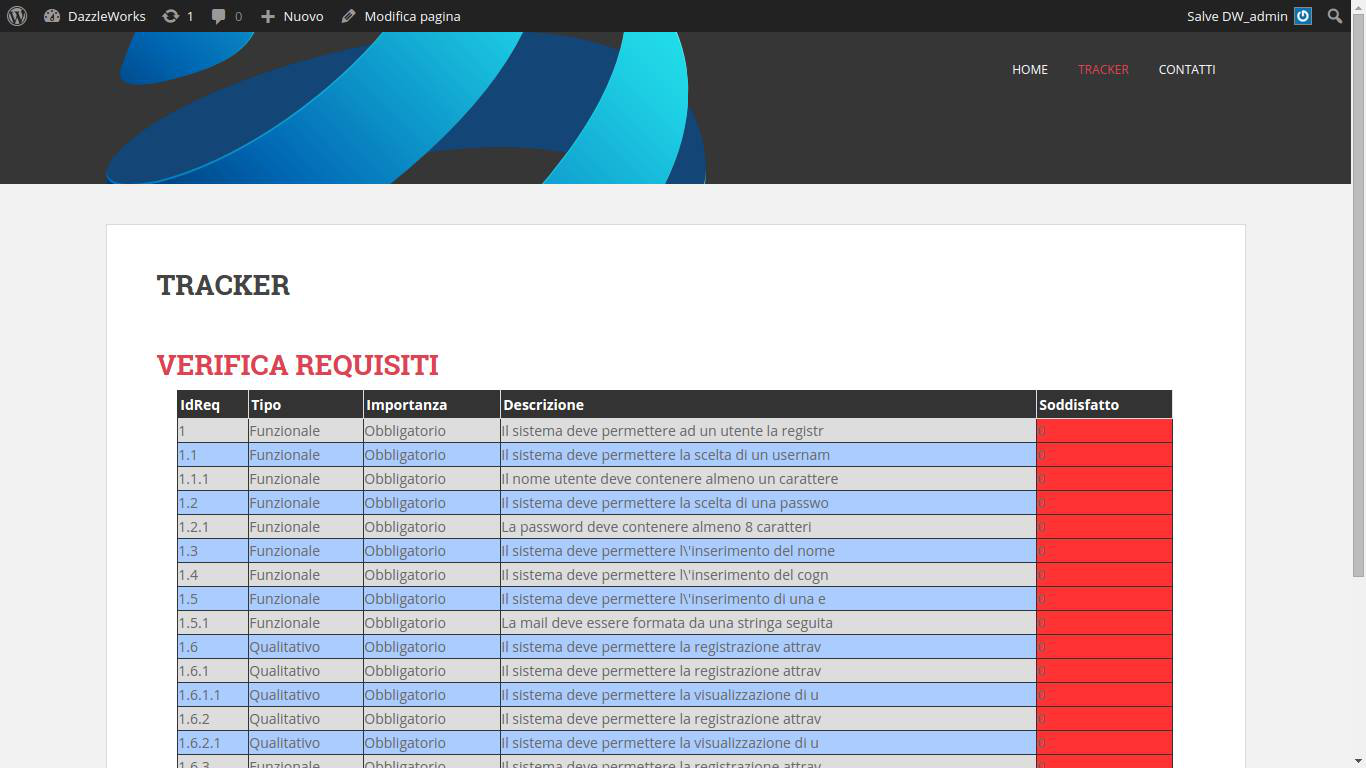
\includegraphics[width=0.7\linewidth]{img/tracker1}
\caption[Pagina riepilogo requisiti]{Pagina riepilogo requisiti}
\label{fig:tracker1}
\end{figure}
\begin{figure}[h]
\centering
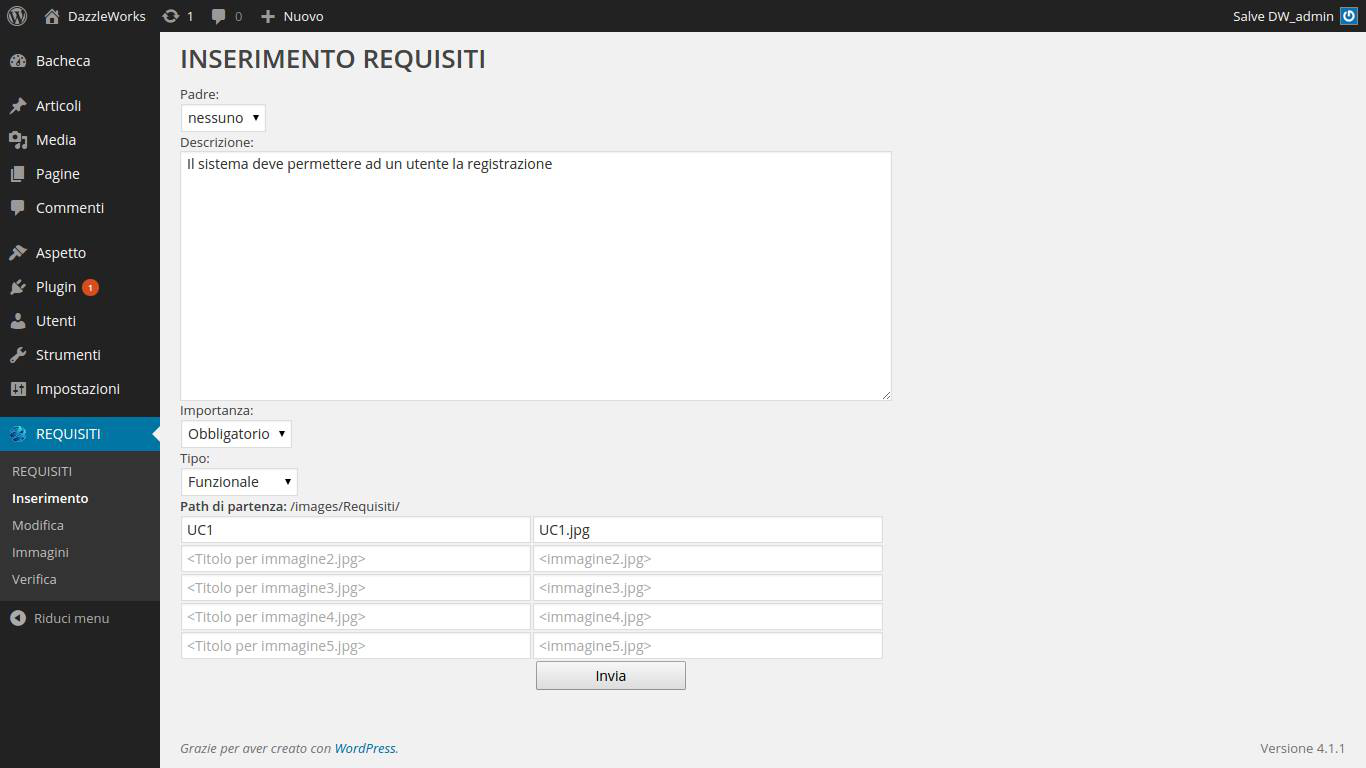
\includegraphics[width=0.7\linewidth]{img/tracker2}
\caption[Pagina inserimento requisito]{Pagina inserimento requisito}
\label{fig:tracker2}
\end{figure}




\newpage
\subsubsection{Progettazione}
Dopo la fase di \textbf{Analisi} si passerà alla fase di \textbf{Progettazione} dove i \textit{Progettisti} dovranno seguire le seguenti regole.\\
\paragraph{Diagrammi UML}
Dovranno essere realizzati i seguenti diagrammi:
\begin{itemize}
	\item Diagrammi delle classi;
	\item Diagrammi dei package;
	\item Diagrammi delle attività;
	\item Diagrammi di sequenza.
\end{itemize}
La lingua utilizzata nella realizzazione dei diagrammi sarà l'\textbf{inglese} e lo standard \gls{UML} sarà 2.0.

\paragraph{Design Pattern}
I \textit{Progettisti} dovranno utilizzare il \gls{design pattern} che ritengono più adatto al contesto per rendere l'applicazione più efficiente possibile. Ogni \gls{design pattern} utilizzato verrà accompagnato da una breve descrizione e da un diagramma che ne esemplifica il funzionamento.

\paragraph{Classi di verifica}
Andranno create delle classi di verifica per testare che tutti i componenti abbiano un comportamento corretto.

\paragraph{Stile di progettazione}
Durante la fase di \textbf{Progettazione} bisognerà fare attenzione a:
\begin{itemize}
	\item \textbf{Ricorsione}: non dovrà essere utilizzata la ricorsione a meno che non sia strettamente necessaria. In quel caso dovrà essere fornita una dimostrazione induttiva sulla correttezza del metodo in questione;
	\item \textbf{Annidamento di cicli}: all'interno di un metodo non dovranno esserci cicli annidati con una profondità maggiore a cinque.
\end{itemize}






\newpage
\subsubsection{Progettazione architetturale}
Lo scopo di questa attività è di fornire un'architettura di alto livello finalizzato ad individuare i sottosistemi che compongono il sistema da realizzare e le loro inter-relazioni di controllo e comunicazione. I compiti principali di questa attività constano nell'individuare le componenti fondamentali e i \gls{design pattern} che serviranno a comporre lo scheletro dell'architettura. Sarà inoltre necessario individuare le componenti esterne che andranno ad interagire con il software e andranno definite di conseguenze le relative interfacce.
 \begin{itemize}
 	\item \textbf{Identificazione dei componenti: }consiste nell'identificazione dei componenti che il sistema software dovrà avere. I \textit{Progettisti} sono tenuti a studiare le migliori strategie implementative, al fine di soddisfarli, e individuare i \gls{design pattern} più adatti;
 	\item \textbf{Identificazione delle interfacce: }consiste nell'identificazione delle interfacce necessarie per la comunicazione con le entità esterne. I \textit{Progettisti} sono tenuti a studiare i possibili componenti esterni;
 	\item \textbf{Documentazione dei documenti: }nel momento dell'individuazione di un componente, è necessario procedere alla stesura della sua documentazione. Ogni package avrà le seguenti caratteristiche:
	 	\begin{itemize}
	 		\item \textbf{Identificativo: }ogni package va tracciato con un nome esaustivo con la prima lettera maiuscola. Di seguito si riporta un esempio con package e sotto-package:
	 		{\centering \textbf{Package::SottoPackage1::SottoPackage2 ...};}
	 		\item \textbf{Diagramma: }ogni package deve essere corredato da un diagramma di package in linguaggio UML;
	 		\item \textbf{Descrizione: }ogni package deve avere una descrizione esauriente;
	 		\item \textbf{Sotto-Package: }ogni package deve essere corredato dalla lista di sotto-package che eventualmente contiene;
	 		\item \textbf{Classi contenute: }ogni package deve essere corredato dalla lista delle classi che eventualmente contiene.
	 	\end{itemize}
	 \item \textbf{Tracciamento dei componenti: }ogni requisito deve essere tracciato al componente che lo soddisfa. Per questo i \textit{Progettisti} sono tenuti a utilizzare l'applicativo \textbf{Tracker} per le varie operazioni di tracciamento.
 \end{itemize}
 
\subsubsection{Progettazione architetturale di dettaglio}
Lo scopo di questa attività è fornire un'architettura sufficientemente dettagliata per permettere la codifica e la stesura dei relativi test di unità. I compiti principali di questa attività constano nell'individuare i metodi delle classi definite durante la progettazione ad alto livello, nella documentazione e nella stesura dei test di unità.
	\begin{itemize}
		\item \textbf{Documentazione delle classi: }ogni classe deve avere le seguenti informazioni:
			\begin{itemize}
				\item \textbf{Diagramma: }diagramma UML che rappresenta la classe;
				\item \textbf{Descrizione: }ogni classe deve avere una descrizione esauriente;
				\item \textbf{Attributi: }devono essere indicati gli attributi della classe con una breve descrizione;
				\item \textbf{Metodi: }devono essere indicati i metodi della classe con una breve descrizione.
			\end{itemize}
		\item \textbf{Definizione test di unità: } i progettisti dovranno provvedere alla creazione di test di unità per verificare il corretto funzionamento di parti di programma permettendo così una precoce individuazione dei bug. I test di unità accurati possono dare una prova certa se un pezzo di codice funziona correttamente, con importanti vantaggi:
			\begin{itemize}
				\item Semplifica le modifiche;
				\item Semplifica l'integrazione;
				\item Supporta la documentazione.
			\end{itemize}
	\end{itemize}

\subsection{Codifica e Convenzioni}
\subsubsection{Linguaggi di codifica}
Dopo un'analisi del capitolato d'appalto e dei requisiti si è deciso che per lo sviluppo del software richiesto si utilizzeranno i linguaggi \gls{HTML5} , \gls{PHP} e \gls{Javascript}.

\subsubsection{Framework e librerie}
Per semplificare la realizzazione della nostra applicazione web si è deciso di utilizzare il \gls{framework} \gls{Angular}, per migliorare le interfacce utente, e la libreria \gls{Chart.js}, utilizzata per generare grafici.

\subsubsection{Convenzioni di codifica}
Di seguito è riportato l'insieme di norme e convenzioni che il gruppo dovrà seguire nella scrittura e documentazione del codice.
L'unica lingua ammessa per i nomi di variabili, metodi e commenti è l'inglese.

\subsubsection{File HTML}

Ogni file \gls{HTML} deve iniziare con il tag <!DOCTYPE html> che serve ad indicare che verrà utilizzata la versione \gls{HTML5}.
Ogni tag deve contenere un id e può contenere una o più classi.
Gli id e le classi dovranno essere contenute in un file .css a parte per mantenere il più possibile la separazione tra \gls{layout} e contenuto.
Le pagine \gls{HTML} devono rispettare gli standard del \gls{W3C}.

\subsubsection{Nomenclatura}
Per l'assegnazione di nomi a variabili, metodi e costanti andranno seguite le seguenti regole:
\begin{itemize}
	\item \textbf{Funzioni:} va utilizzata la notazione mixed case, con la prima lettera minuscola;
	\item \textbf{Variabili:} va utilizzata la notazione mixed case, con la prima lettera minuscola;
	\item \textbf{Costanti:} va scritto il nome interamente in maiuscolo, separando le varie parole con il carattere "\_" (underscore).
\end{itemize}

\subsubsection{Intestazione di un file Javascript}

\begin{flushleft}

/*\\
\vspace{3mm}
\begin{tabular}{l}
	File\\
	Autore\\
	Data\\
	Descrizione\\
\end{tabular}\\
\vspace{5mm}
 Modifiche:\\
 \vspace{3mm}
\begin{tabular}{| c c c c c c c c c |}
	\hline
	Versione & - & Data & - & Programmatore & - & Modifica & - & Descrizione\\
	\hline
	x.y.z & - & aaaa-mm-gg & - & Nome Cognome & - & Funzione & - & Descrizione modifica\\
	\hline
\end{tabular}\\
\vspace{3mm}
*/\\

\end{flushleft}

\begin{itemize}
	\item \textbf{File:} nome del file;
	\item \textbf{Autore:} nome e cognome del creatore del file;
	\item \textbf{Data:} data di creazione del file nel formato aaaa-mm-gg;
	\item \textbf{Descrizione:} poche righe di descrizione delle funzionalità contenute nel file;
	\item \textbf{Cambiamenti:} tabella dello stato di avanzamento del file, contenente tutte le modifiche effettuate :
		\begin{itemize}
			\item \textbf{Versione:} versione una volta effettuata la modifica;
			\item \textbf{Data:} data della modifica;
			\item \textbf{Programmatore:} nome e cognome del programmatore che ha effettuato la modifica;
			\item \textbf{Modifica:} segnatura della funzione a cui è stata apportata una modifica;
			\item \textbf{Descrizione:} breve descrizione della modifica effettuata.
		\end{itemize}
\end{itemize}

\subsubsection{Commenti}

Prima di ogni funzione dovrà essere presente un commento con la seguente forma:

\begin{flushleft}
/*\\
\vspace{3mm}
\begin{tabular}{l}
	Descrizione della funzione\\
	Descrizione dei parametri\\		
	Descrizione del tipo di ritorno\\
\end{tabular}\\
\vspace{3mm}
*/

\end{flushleft}

Ogni variabile di particolare importanza dovrà essere fornita di commento che ne spieghi scopo e funzionamento.




